\documentclass[12pt]{article}
\usepackage[utf8]{inputenc}
\usepackage[T1]{fontenc}
\usepackage{pdflscape} 
\usepackage{lmodern}
\usepackage[a4paper,bindingoffset=0.2in,%
            left=0.5in,right=0.5in,top=0.5in,bottom=1in,%
            footskip=.25in]{geometry}
\usepackage[colorlinks=true, linkcolor=Black, urlcolor=Blue]{hyperref}
\usepackage{graphicx}
\usepackage{subcaption}
\usepackage{listings}
\usepackage{color}
\usepackage[table]{xcolor}
\definecolor{lightgray}{gray}{0.9}

\definecolor{codegreen}{rgb}{0,0.6,0}
\definecolor{codegray}{rgb}{0.5,0.5,0.5}
\definecolor{codepurple}{rgb}{0.58,0,0.82}
\definecolor{backcolour}{rgb}{0.95,0.95,0.92}

\lstdefinestyle{mystyle}{
	backgroundcolor=\color{backcolour},   
	commentstyle=\color{codegreen},
	keywordstyle=\color{magenta},
	numberstyle=\tiny\color{codegray},
	stringstyle=\color{codepurple},
	basicstyle=\ttfamily\footnotesize,
	breakatwhitespace=false,         
	breaklines=true,                 
	captionpos=b,                    
	keepspaces=true,                 
	numbers=left,                    
	numbersep=5pt,                  
	showspaces=false,                
	showstringspaces=false,
	showtabs=false,                  
	tabsize=2
}


\begin{document}
\title{Projekt - Drzewa Decyzyjne II\\
\large Sebastian Michoń 136770, Marcin Zatorski 136834\\
\large grupe L5}
\date{\vspace{-10ex}}
\maketitle

\section{Wybrane najważniejsze atrybuty}
\begin{enumerate}
	\item sex - nawet jeśli płeć sama w sobie może nie być dobrze skorelowana z tym, czy student zdał, wpływa ona na to, jak dany atrybut wpływa na studenta - np. dla mężczyzn wyższą korelację z wynikiem końcowym może mieć chęć podjęcia edukacji wyższej raczej niż zdrowie, dla kobiet - wręcz przeciwnie.
	
	\item reason - to, dlaczego student wybrał daną szkołę.
	\item failures
	\item higher
	\item Dalc - dzienne spożycie alkoholu w dni robocze
	\item health
	\item absences	
\end{enumerate}

\section{Wybrane metryki}
\begin{enumerate}
	\item Accuracy - jako, że dataset jest dosyć zrównoważony (115/85 dla zestawu treningowego i 118/77 dla testowego) wykorzystanie procentu trafień jest zasadne.
	\item F1 measure - jeśli jakaś inna miara poza celnością jest zasadna, to najprędzej F1 - pozwala ona bowiem zagregować informację o precyzji i czułości
	\item Ostatnią miarą, która zostanie użyta jest Balanced accuracy - \(\frac{TPR+TNR}{2}\), czyli suma czułości i selektywności podzielona przez przez 2 - nieco lepsza niż Accuracy, jako że proporcja w tym datasecie to 3:2 (gdzie więcej osób nie zdało niż zdało)
\end{enumerate}


\section{Rezultaty 3 wywołań algorytmu J48 (algorytm drzewa decyzyjnego z Weki) w zależności od datasetu, liczby atrybutów i techniki ewaluacji}
\clearpage
	\rowcolors{2}{gray!25}{white}
	\begin{table}
		\caption{Porównanie wartości wybranych metryk dla drzew decyzyjnych trenowanych na wybranych atrybutach - math dataset, zadanie 4.}
		\scalebox{0.64}{
		\begin{tabular}{| l | l | l | l | l | l | l | l | l | l |}
			\rowcolor{gray!50}
			\hline
			Binary Split & Confidence factor & Minimum objects & TP & FP & FN & TN & Accuracy & F1 & Balanced Accuracy\\ \hline
			0 & 0.1000 & 2 & 31 & 37 & 46 & 81 & 0.5744 & 0.4276 & 0.5445\\ \hline
			0 & 0.2000 & 2 & 31 & 37 & 46 & 81 & 0.5744 & 0.4276 & 0.5445\\ \hline
			0 & 0.3000 & 2 & 31 & 37 & 46 & 81 & 0.5744 & 0.4276 & 0.5445\\ \hline
			0 & 0.4000 & 2 & 31 & 37 & 46 & 81 & 0.5744 & 0.4276 & 0.5445\\ \hline
			0 & 0.5000 & 2 & 27 & 28 & 50 & 90 & 0.6000 & 0.4091 & 0.5567\\ \hline
			0 & 0.6000 & 2 & 28 & 35 & 49 & 83 & 0.5692 & 0.4000 & 0.5335\\ \hline
			0 & 0.7000 & 2 & 28 & 35 & 49 & 83 & 0.5692 & 0.4000 & 0.5335\\ \hline
			0 & 0.8000 & 2 & 28 & 35 & 49 & 83 & 0.5692 & 0.4000 & 0.5335\\ \hline
			0 & 0.9000 & 2 & 28 & 35 & 49 & 83 & 0.5692 & 0.4000 & 0.5335\\ \hline
			1 & 0.1000 & 2 & 31 & 37 & 46 & 81 & 0.5744 & 0.4276 & 0.5445\\ \hline
			1 & 0.2000 & 2 & 31 & 37 & 46 & 81 & 0.5744 & 0.4276 & 0.5445\\ \hline
			1 & 0.3000 & 2 & 27 & 29 & 50 & 89 & 0.5949 & 0.4060 & 0.5524\\ \hline
			1 & 0.4000 & 2 & 26 & 23 & 51 & 95 & 0.6205 & 0.4127 & 0.5714\\ \hline
			1 & 0.5000 & 2 & 26 & 23 & 51 & 95 & 0.6205 & 0.4127 & 0.5714\\ \hline
			1 & 0.6000 & 2 & 30 & 30 & 47 & 88 & 0.6051 & 0.4380 & 0.5677\\ \hline
			1 & 0.7000 & 2 & 30 & 30 & 47 & 88 & 0.6051 & 0.4380 & 0.5677\\ \hline
			1 & 0.8000 & 2 & 30 & 30 & 47 & 88 & 0.6051 & 0.4380 & 0.5677\\ \hline
			1 & 0.9000 & 2 & 30 & 30 & 47 & 88 & 0.6051 & 0.4380 & 0.5677\\ \hline
			0 & 0.1000 & 3 & 31 & 37 & 46 & 81 & 0.5744 & 0.4276 & 0.5445\\ \hline
			0 & 0.2000 & 3 & 31 & 37 & 46 & 81 & 0.5744 & 0.4276 & 0.5445\\ \hline
			0 & 0.3000 & 3 & 31 & 37 & 46 & 81 & 0.5744 & 0.4276 & 0.5445\\ \hline
			0 & 0.4000 & 3 & 31 & 37 & 46 & 81 & 0.5744 & 0.4276 & 0.5445\\ \hline
			0 & 0.5000 & 3 & 23 & 27 & 54 & 91 & 0.5846 & 0.3622 & 0.5349\\ \hline
			0 & 0.6000 & 3 & 24 & 34 & 53 & 84 & 0.5538 & 0.3556 & 0.5118\\ \hline
			0 & 0.7000 & 3 & 24 & 34 & 53 & 84 & 0.5538 & 0.3556 & 0.5118\\ \hline
			0 & 0.8000 & 3 & 24 & 34 & 53 & 84 & 0.5538 & 0.3556 & 0.5118\\ \hline
			0 & 0.9000 & 3 & 24 & 34 & 53 & 84 & 0.5538 & 0.3556 & 0.5118\\ \hline
			1 & 0.1000 & 3 & 31 & 37 & 46 & 81 & 0.5744 & 0.4276 & 0.5445\\ \hline
			1 & 0.2000 & 3 & 31 & 37 & 46 & 81 & 0.5744 & 0.4276 & 0.5445\\ \hline
			1 & 0.3000 & 3 & 31 & 37 & 46 & 81 & 0.5744 & 0.4276 & 0.5445\\ \hline
			1 & 0.4000 & 3 & 25 & 29 & 52 & 89 & 0.5846 & 0.3817 & 0.5395\\ \hline
			1 & 0.5000 & 3 & 25 & 25 & 52 & 93 & 0.6051 & 0.3937 & 0.5564\\ \hline
			1 & 0.6000 & 3 & 28 & 28 & 49 & 90 & 0.6051 & 0.4211 & 0.5632\\ \hline
			1 & 0.7000 & 3 & 28 & 28 & 49 & 90 & 0.6051 & 0.4211 & 0.5632\\ \hline
			1 & 0.8000 & 3 & 28 & 28 & 49 & 90 & 0.6051 & 0.4211 & 0.5632\\ \hline
			1 & 0.9000 & 3 & 28 & 28 & 49 & 90 & 0.6051 & 0.4211 & 0.5632\\ \hline
			0 & 0.1000 & 4 & 31 & 37 & 46 & 81 & 0.5744 & 0.4276 & 0.5445\\ \hline
			0 & 0.2000 & 4 & 31 & 37 & 46 & 81 & 0.5744 & 0.4276 & 0.5445\\ \hline
			0 & 0.3000 & 4 & 31 & 37 & 46 & 81 & 0.5744 & 0.4276 & 0.5445\\ \hline
			0 & 0.4000 & 4 & 31 & 37 & 46 & 81 & 0.5744 & 0.4276 & 0.5445\\ \hline
			0 & 0.5000 & 4 & 31 & 37 & 46 & 81 & 0.5744 & 0.4276 & 0.5445\\ \hline
			0 & 0.6000 & 4 & 25 & 27 & 52 & 91 & 0.5949 & 0.3876 & 0.5479\\ \hline
			0 & 0.7000 & 4 & 25 & 27 & 52 & 91 & 0.5949 & 0.3876 & 0.5479\\ \hline
			0 & 0.8000 & 4 & 25 & 27 & 52 & 91 & 0.5949 & 0.3876 & 0.5479\\ \hline
			0 & 0.9000 & 4 & 25 & 27 & 52 & 91 & 0.5949 & 0.3876 & 0.5479\\ \hline
			1 & 0.1000 & 4 & 31 & 37 & 46 & 81 & 0.5744 & 0.4276 & 0.5445\\ \hline
			1 & 0.2000 & 4 & 31 & 37 & 46 & 81 & 0.5744 & 0.4276 & 0.5445\\ \hline
			1 & 0.3000 & 4 & 25 & 28 & 52 & 90 & 0.5897 & 0.3846 & 0.5437\\ \hline
			1 & 0.4000 & 4 & 25 & 28 & 52 & 90 & 0.5897 & 0.3846 & 0.5437\\ \hline
			1 & 0.5000 & 4 & 25 & 24 & 52 & 94 & 0.6103 & 0.3968 & 0.5606\\ \hline
			1 & 0.6000 & 4 & 25 & 24 & 52 & 94 & 0.6103 & 0.3968 & 0.5606\\ \hline
			1 & 0.7000 & 4 & 25 & 24 & 52 & 94 & 0.6103 & 0.3968 & 0.5606\\ \hline
			1 & 0.8000 & 4 & 25 & 24 & 52 & 94 & 0.6103 & 0.3968 & 0.5606\\ \hline
			1 & 0.9000 & 4 & 25 & 24 & 52 & 94 & 0.6103 & 0.3968 & 0.5606\\ \hline
			0 & 0.1000 & 5 & 40 & 53 & 37 & 65 & 0.5385 & 0.4706 & 0.5352\\ \hline
			0 & 0.2000 & 5 & 19 & 16 & 58 & 102 & 0.6205 & 0.3393 & 0.5556\\ \hline
			0 & 0.3000 & 5 & 19 & 16 & 58 & 102 & 0.6205 & 0.3393 & 0.5556\\ \hline
			0 & 0.4000 & 5 & 19 & 16 & 58 & 102 & 0.6205 & 0.3393 & 0.5556\\ \hline
			0 & 0.5000 & 5 & 19 & 16 & 58 & 102 & 0.6205 & 0.3393 & 0.5556\\ \hline
			0 & 0.6000 & 5 & 19 & 16 & 58 & 102 & 0.6205 & 0.3393 & 0.5556\\ \hline
			0 & 0.7000 & 5 & 19 & 16 & 58 & 102 & 0.6205 & 0.3393 & 0.5556\\ \hline
			0 & 0.8000 & 5 & 19 & 16 & 58 & 102 & 0.6205 & 0.3393 & 0.5556\\ \hline
			0 & 0.9000 & 5 & 19 & 16 & 58 & 102 & 0.6205 & 0.3393 & 0.5556\\ \hline
			1 & 0.1000 & 5 & 36 & 49 & 41 & 69 & 0.5385 & 0.4444 & 0.5261\\ \hline
			1 & 0.2000 & 5 & 22 & 18 & 55 & 100 & 0.6256 & 0.3761 & 0.5666\\ \hline
			1 & 0.3000 & 5 & 24 & 27 & 53 & 91 & 0.5897 & 0.3750 & 0.5414\\ \hline
			1 & 0.4000 & 5 & 24 & 27 & 53 & 91 & 0.5897 & 0.3750 & 0.5414\\ \hline
			1 & 0.5000 & 5 & 24 & 27 & 53 & 91 & 0.5897 & 0.3750 & 0.5414\\ \hline
			1 & 0.6000 & 5 & 24 & 27 & 53 & 91 & 0.5897 & 0.3750 & 0.5414\\ \hline
			1 & 0.7000 & 5 & 24 & 27 & 53 & 91 & 0.5897 & 0.3750 & 0.5414\\ \hline
			1 & 0.8000 & 5 & 24 & 27 & 53 & 91 & 0.5897 & 0.3750 & 0.5414\\ \hline
			1 & 0.9000 & 5 & 24 & 27 & 53 & 91 & 0.5897 & 0.3750 & 0.5414\\ \hline
			
		\end{tabular}
	}
	\end{table}
\clearpage
\begin{figure}[h!]
	\centering
	\begin{subfigure}[b]{1\linewidth}
		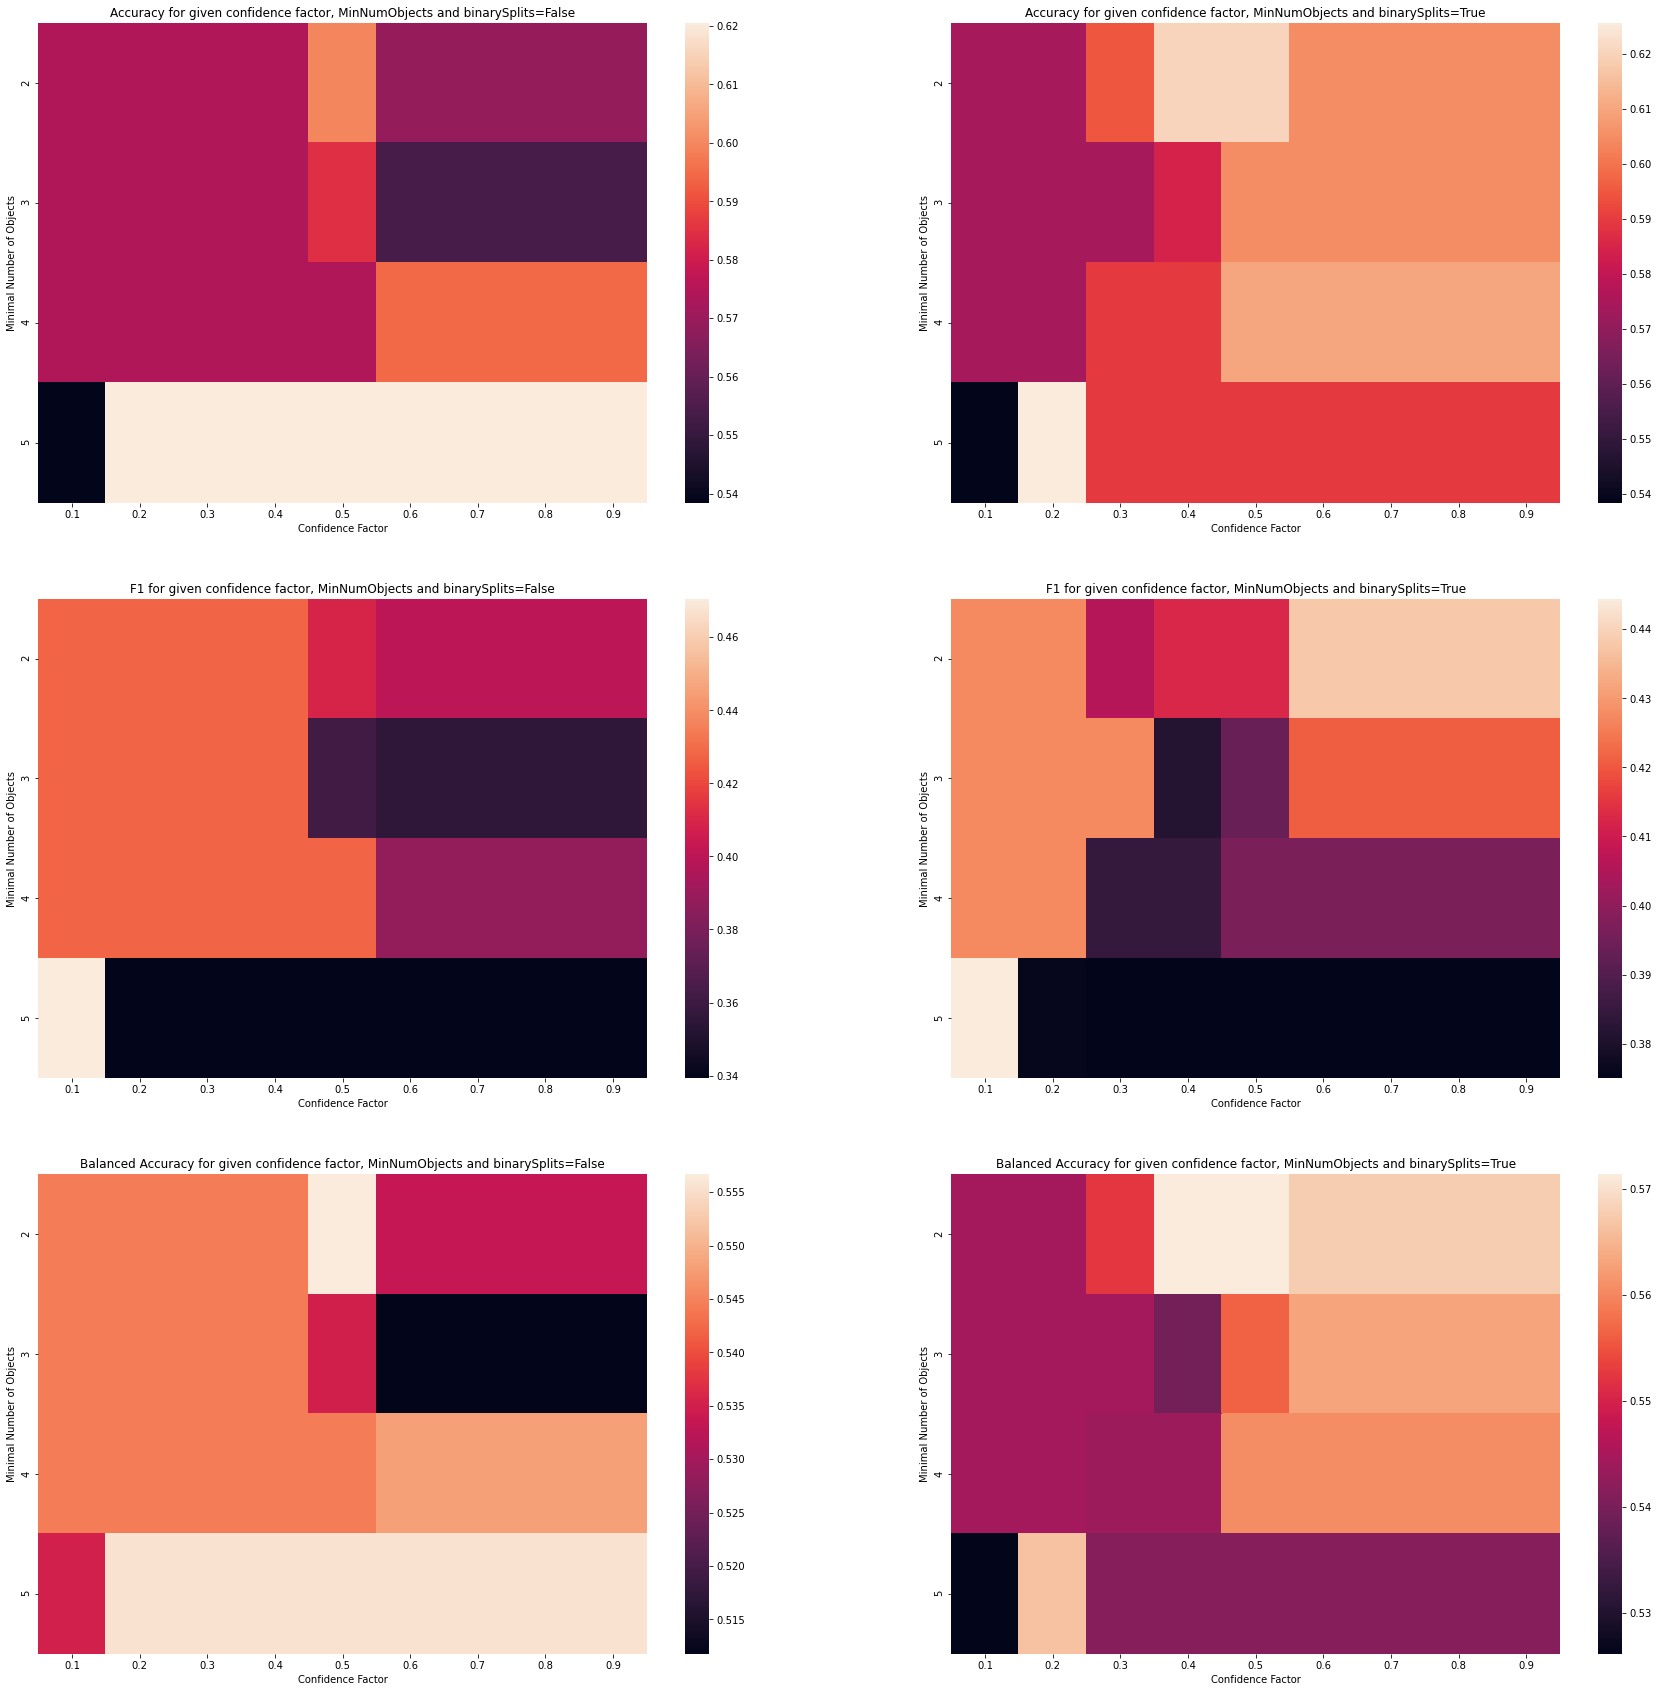
\includegraphics[width=\linewidth]{Train_sub.png}
	\end{subfigure}
	\label{fig:Chosen}
	\caption{Wartość kolejnych metryk w zależności od hiperparametrów: Confidence factor i Minimum number of objects (in a leaf) - zadanie 4.}
\end{figure}

\clearpage
\begin{figure}[h!]
	\centering
	\begin{subfigure}[b]{1\linewidth}
		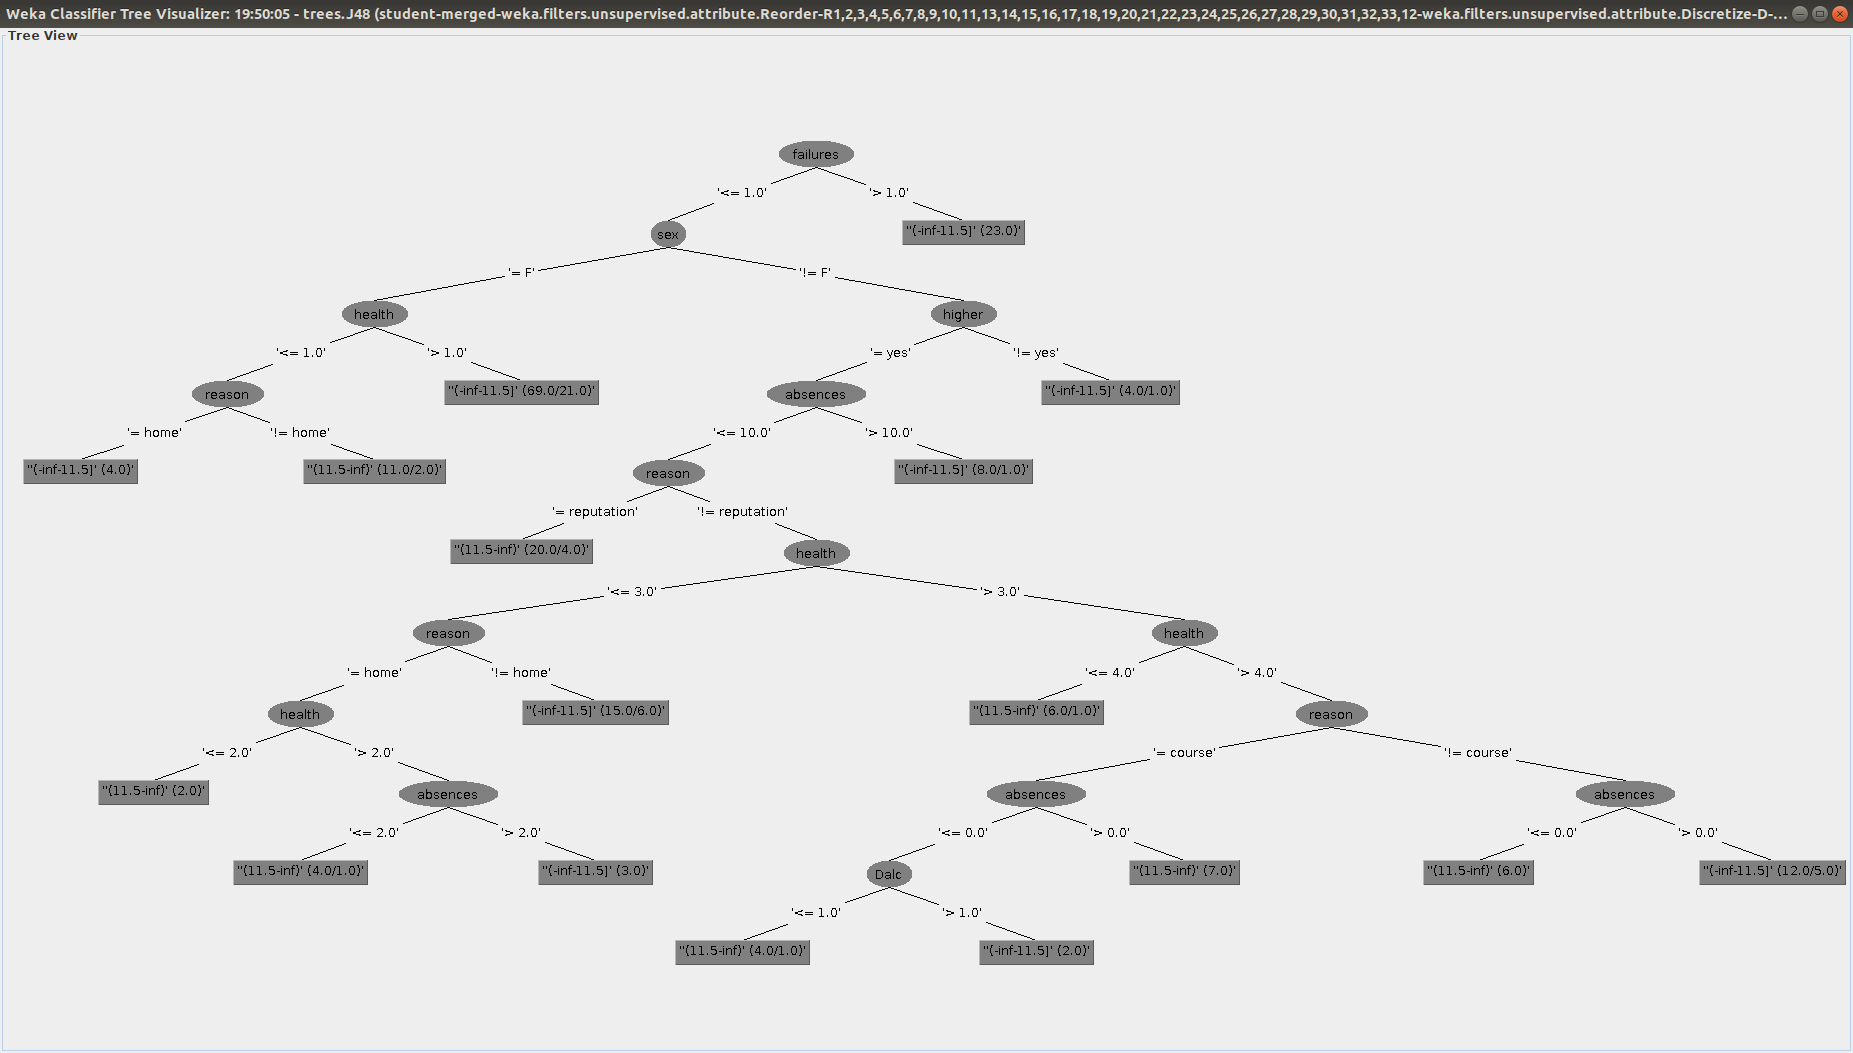
\includegraphics[width=\linewidth]{Drzewo_train_sub.png}
	\end{subfigure}
	\label{fig:ChosenNext}
	\caption{Najlepsze drzewo - ConfidenceFactor=0.5, MinNumbObj=2, BinarySplit=True - zadanie 4.}
\end{figure}


\clearpage
\rowcolors{2}{gray!25}{white}
\begin{table}
	\caption{Porównanie wartości wybranych metryk dla drzew decyzyjnych trenowanych na wszystkich atrybutach - math dataset, zadanie 5.}
	\scalebox{0.64}{
		\begin{tabular}{| l | l | l | l | l | l | l | l | l | l |}
			\rowcolor{gray!50}
			\hline
			Binary Split & Confidence factor & Minimum objects & TP & FP & FN & TN & Accuracy & F1 & Balanced Accuracy\\ \hline
			0 & 0.1000 & 2 & 29 & 48 & 48 & 70 & 0.5077 & 0.3766 & 0.4849\\ \hline
			0 & 0.2000 & 2 & 29 & 48 & 48 & 70 & 0.5077 & 0.3766 & 0.4849\\ \hline
			0 & 0.3000 & 2 & 29 & 48 & 48 & 70 & 0.5077 & 0.3766 & 0.4849\\ \hline
			0 & 0.4000 & 2 & 29 & 49 & 48 & 69 & 0.5026 & 0.3742 & 0.4807\\ \hline
			0 & 0.5000 & 2 & 28 & 49 & 49 & 69 & 0.4974 & 0.3636 & 0.4742\\ \hline
			0 & 0.6000 & 2 & 28 & 49 & 49 & 69 & 0.4974 & 0.3636 & 0.4742\\ \hline
			0 & 0.7000 & 2 & 28 & 49 & 49 & 69 & 0.4974 & 0.3636 & 0.4742\\ \hline
			0 & 0.8000 & 2 & 28 & 49 & 49 & 69 & 0.4974 & 0.3636 & 0.4742\\ \hline
			0 & 0.9000 & 2 & 28 & 49 & 49 & 69 & 0.4974 & 0.3636 & 0.4742\\ \hline
			1 & 0.1000 & 2 & 36 & 41 & 41 & 77 & 0.5795 & 0.4675 & 0.5600\\ \hline
			1 & 0.2000 & 2 & 36 & 41 & 41 & 77 & 0.5795 & 0.4675 & 0.5600\\ \hline
			1 & 0.3000 & 2 & 37 & 48 & 40 & 70 & 0.5487 & 0.4568 & 0.5369\\ \hline
			1 & 0.4000 & 2 & 37 & 48 & 40 & 70 & 0.5487 & 0.4568 & 0.5369\\ \hline
			1 & 0.5000 & 2 & 37 & 48 & 40 & 70 & 0.5487 & 0.4568 & 0.5369\\ \hline
			1 & 0.6000 & 2 & 36 & 47 & 41 & 71 & 0.5487 & 0.4500 & 0.5346\\ \hline
			1 & 0.7000 & 2 & 36 & 47 & 41 & 71 & 0.5487 & 0.4500 & 0.5346\\ \hline
			1 & 0.8000 & 2 & 36 & 47 & 41 & 71 & 0.5487 & 0.4500 & 0.5346\\ \hline
			1 & 0.9000 & 2 & 36 & 47 & 41 & 71 & 0.5487 & 0.4500 & 0.5346\\ \hline
			0 & 0.1000 & 3 & 29 & 48 & 48 & 70 & 0.5077 & 0.3766 & 0.4849\\ \hline
			0 & 0.2000 & 3 & 29 & 48 & 48 & 70 & 0.5077 & 0.3766 & 0.4849\\ \hline
			0 & 0.3000 & 3 & 29 & 48 & 48 & 70 & 0.5077 & 0.3766 & 0.4849\\ \hline
			0 & 0.4000 & 3 & 29 & 48 & 48 & 70 & 0.5077 & 0.3766 & 0.4849\\ \hline
			0 & 0.5000 & 3 & 28 & 48 & 49 & 70 & 0.5026 & 0.3660 & 0.4784\\ \hline
			0 & 0.6000 & 3 & 28 & 48 & 49 & 70 & 0.5026 & 0.3660 & 0.4784\\ \hline
			0 & 0.7000 & 3 & 28 & 48 & 49 & 70 & 0.5026 & 0.3660 & 0.4784\\ \hline
			0 & 0.8000 & 3 & 28 & 48 & 49 & 70 & 0.5026 & 0.3660 & 0.4784\\ \hline
			0 & 0.9000 & 3 & 28 & 48 & 49 & 70 & 0.5026 & 0.3660 & 0.4784\\ \hline
			1 & 0.1000 & 3 & 40 & 42 & 37 & 76 & 0.5949 & 0.5031 & 0.5818\\ \hline
			1 & 0.2000 & 3 & 41 & 44 & 36 & 74 & 0.5897 & 0.5062 & 0.5798\\ \hline
			1 & 0.3000 & 3 & 42 & 36 & 35 & 82 & 0.6359 & 0.5419 & 0.6202\\ \hline
			1 & 0.4000 & 3 & 41 & 33 & 36 & 85 & 0.6462 & 0.5430 & 0.6264\\ \hline
			1 & 0.5000 & 3 & 41 & 33 & 36 & 85 & 0.6462 & 0.5430 & 0.6264\\ \hline
			1 & 0.6000 & 3 & 37 & 32 & 40 & 86 & 0.6308 & 0.5068 & 0.6047\\ \hline
			1 & 0.7000 & 3 & 37 & 32 & 40 & 86 & 0.6308 & 0.5068 & 0.6047\\ \hline
			1 & 0.8000 & 3 & 37 & 32 & 40 & 86 & 0.6308 & 0.5068 & 0.6047\\ \hline
			1 & 0.9000 & 3 & 37 & 32 & 40 & 86 & 0.6308 & 0.5068 & 0.6047\\ \hline
			0 & 0.1000 & 4 & 14 & 30 & 63 & 88 & 0.5231 & 0.2314 & 0.4638\\ \hline
			0 & 0.2000 & 4 & 14 & 28 & 63 & 90 & 0.5333 & 0.2353 & 0.4723\\ \hline
			0 & 0.3000 & 4 & 14 & 28 & 63 & 90 & 0.5333 & 0.2353 & 0.4723\\ \hline
			0 & 0.4000 & 4 & 14 & 28 & 63 & 90 & 0.5333 & 0.2353 & 0.4723\\ \hline
			0 & 0.5000 & 4 & 14 & 28 & 63 & 90 & 0.5333 & 0.2353 & 0.4723\\ \hline
			0 & 0.6000 & 4 & 14 & 28 & 63 & 90 & 0.5333 & 0.2353 & 0.4723\\ \hline
			0 & 0.7000 & 4 & 14 & 28 & 63 & 90 & 0.5333 & 0.2353 & 0.4723\\ \hline
			0 & 0.8000 & 4 & 14 & 28 & 63 & 90 & 0.5333 & 0.2353 & 0.4723\\ \hline
			0 & 0.9000 & 4 & 14 & 28 & 63 & 90 & 0.5333 & 0.2353 & 0.4723\\ \hline
			1 & 0.1000 & 4 & 31 & 41 & 46 & 77 & 0.5538 & 0.4161 & 0.5276\\ \hline
			1 & 0.2000 & 4 & 28 & 39 & 49 & 79 & 0.5487 & 0.3889 & 0.5166\\ \hline
			1 & 0.3000 & 4 & 28 & 39 & 49 & 79 & 0.5487 & 0.3889 & 0.5166\\ \hline
			1 & 0.4000 & 4 & 33 & 40 & 44 & 78 & 0.5692 & 0.4400 & 0.5448\\ \hline
			1 & 0.5000 & 4 & 33 & 40 & 44 & 78 & 0.5692 & 0.4400 & 0.5448\\ \hline
			1 & 0.6000 & 4 & 33 & 40 & 44 & 78 & 0.5692 & 0.4400 & 0.5448\\ \hline
			1 & 0.7000 & 4 & 33 & 40 & 44 & 78 & 0.5692 & 0.4400 & 0.5448\\ \hline
			1 & 0.8000 & 4 & 33 & 40 & 44 & 78 & 0.5692 & 0.4400 & 0.5448\\ \hline
			1 & 0.9000 & 4 & 33 & 40 & 44 & 78 & 0.5692 & 0.4400 & 0.5448\\ \hline
			0 & 0.1000 & 5 & 13 & 30 & 64 & 88 & 0.5179 & 0.2167 & 0.4573\\ \hline
			0 & 0.2000 & 5 & 12 & 31 & 65 & 87 & 0.5077 & 0.2000 & 0.4466\\ \hline
			0 & 0.3000 & 5 & 12 & 31 & 65 & 87 & 0.5077 & 0.2000 & 0.4466\\ \hline
			0 & 0.4000 & 5 & 13 & 31 & 64 & 87 & 0.5128 & 0.2149 & 0.4531\\ \hline
			0 & 0.5000 & 5 & 13 & 31 & 64 & 87 & 0.5128 & 0.2149 & 0.4531\\ \hline
			0 & 0.6000 & 5 & 13 & 29 & 64 & 89 & 0.5231 & 0.2185 & 0.4615\\ \hline
			0 & 0.7000 & 5 & 13 & 29 & 64 & 89 & 0.5231 & 0.2185 & 0.4615\\ \hline
			0 & 0.8000 & 5 & 13 & 29 & 64 & 89 & 0.5231 & 0.2185 & 0.4615\\ \hline
			0 & 0.9000 & 5 & 13 & 29 & 64 & 89 & 0.5231 & 0.2185 & 0.4615\\ \hline
			1 & 0.1000 & 5 & 35 & 46 & 42 & 72 & 0.5487 & 0.4430 & 0.5324\\ \hline
			1 & 0.2000 & 5 & 35 & 46 & 42 & 72 & 0.5487 & 0.4430 & 0.5324\\ \hline
			1 & 0.3000 & 5 & 29 & 37 & 48 & 81 & 0.5641 & 0.4056 & 0.5315\\ \hline
			1 & 0.4000 & 5 & 34 & 38 & 43 & 80 & 0.5846 & 0.4564 & 0.5598\\ \hline
			1 & 0.5000 & 5 & 34 & 38 & 43 & 80 & 0.5846 & 0.4564 & 0.5598\\ \hline
			1 & 0.6000 & 5 & 34 & 38 & 43 & 80 & 0.5846 & 0.4564 & 0.5598\\ \hline
			1 & 0.7000 & 5 & 34 & 38 & 43 & 80 & 0.5846 & 0.4564 & 0.5598\\ \hline
			1 & 0.8000 & 5 & 34 & 38 & 43 & 80 & 0.5846 & 0.4564 & 0.5598\\ \hline
			1 & 0.9000 & 5 & 34 & 38 & 43 & 80 & 0.5846 & 0.4564 & 0.5598\\ \hline
		\end{tabular}
	}
\end{table}
\clearpage

\begin{figure}[h!]
	\centering
	\begin{subfigure}[b]{1\linewidth}
		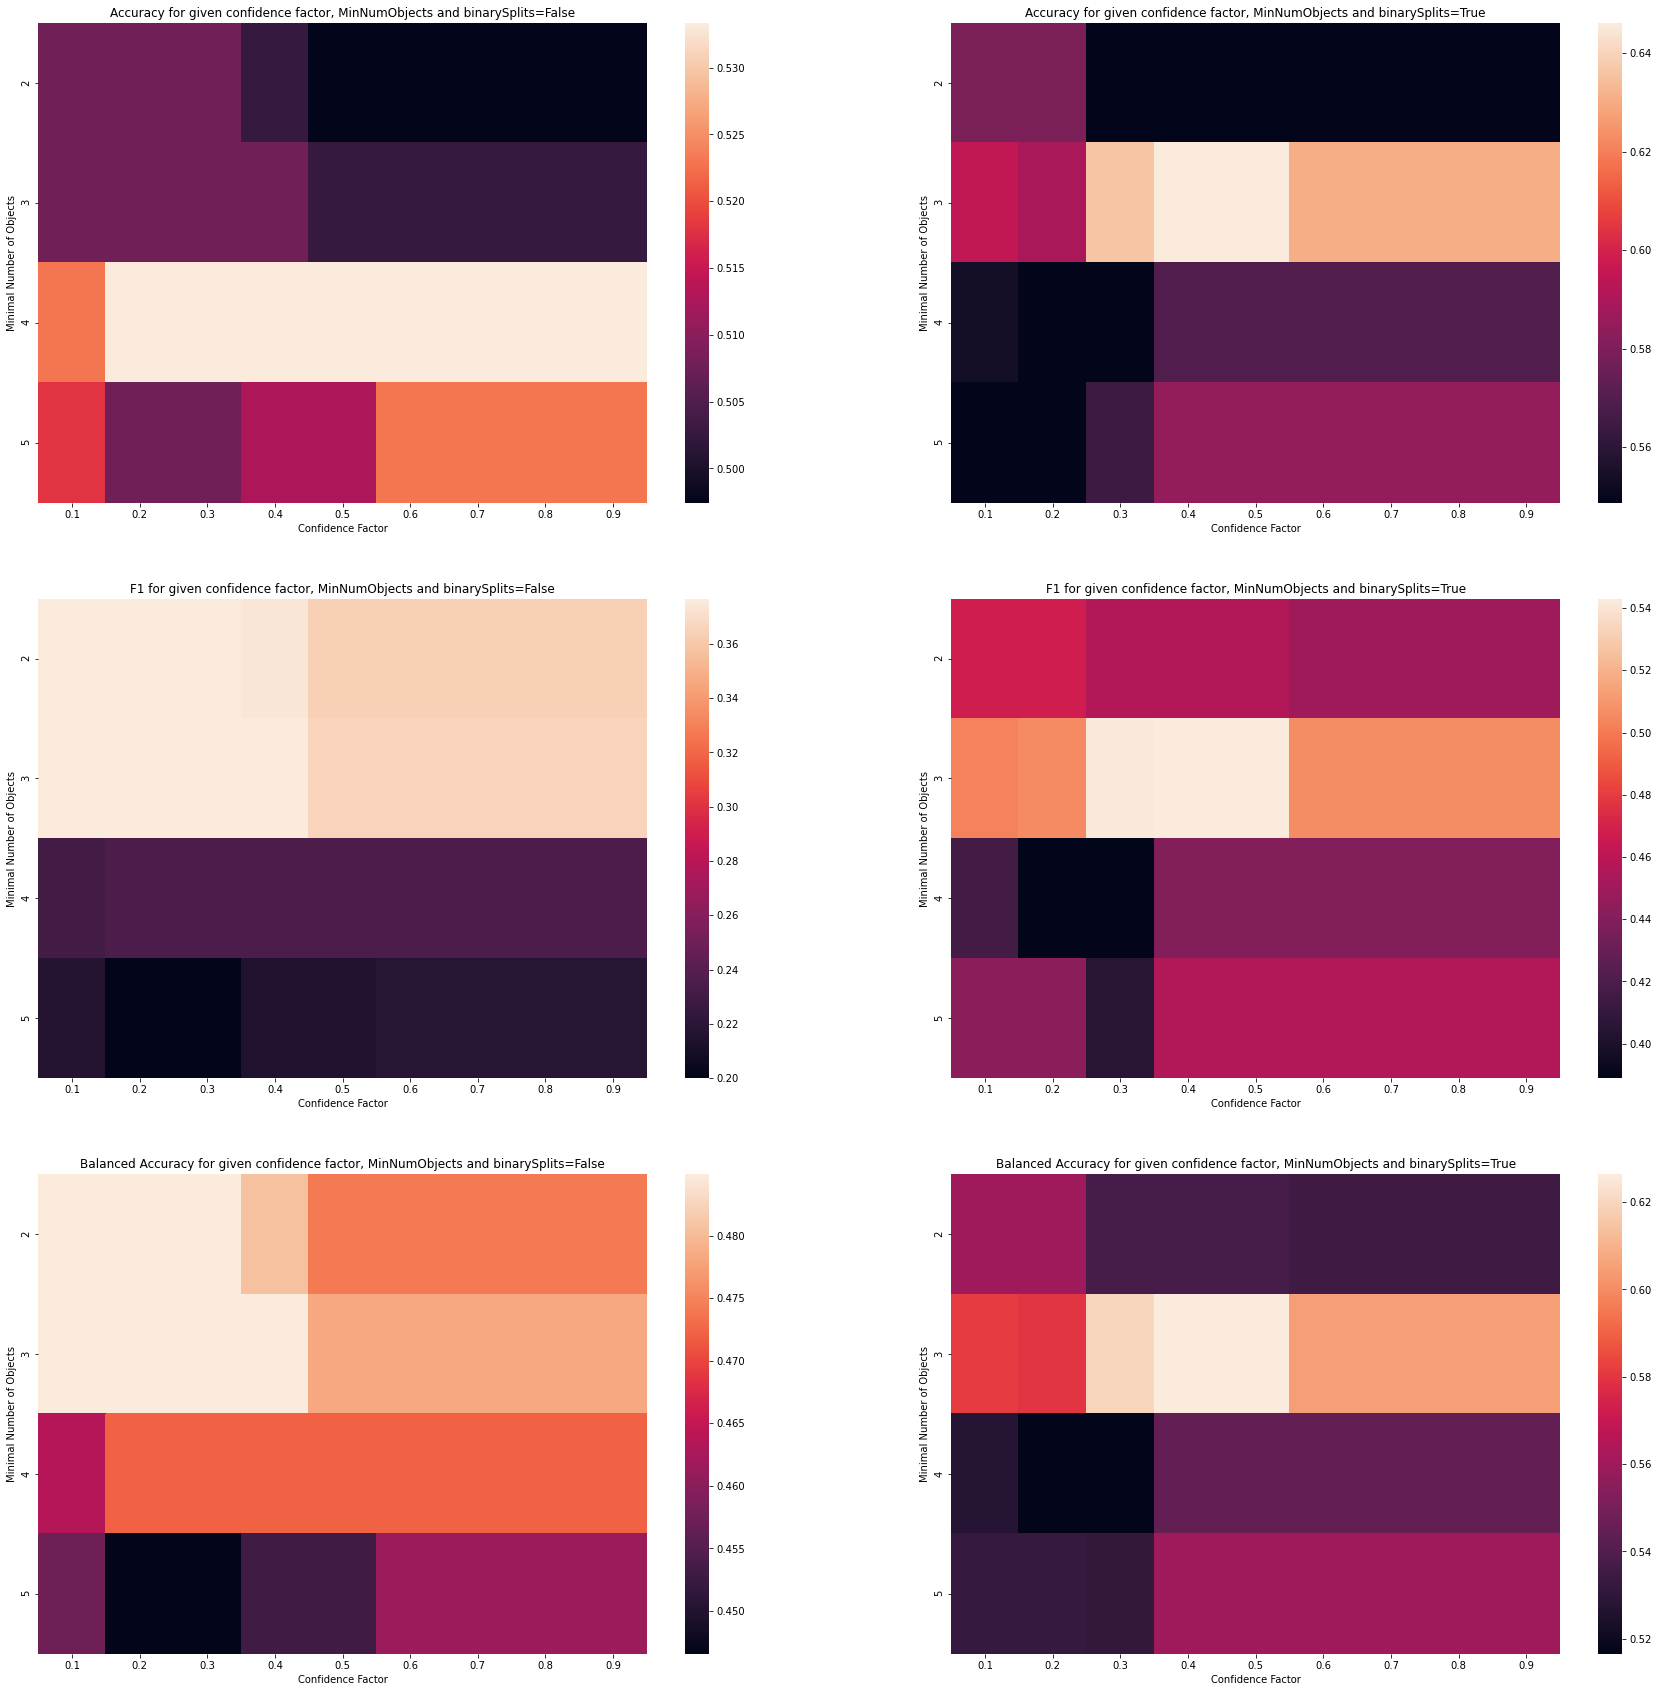
\includegraphics[width=\linewidth]{Train_All.png}
	\end{subfigure}
	\label{fig:Chosen}
	\caption{Wartość kolejnych metryk w zależności od hiperparametrów: Confidence factor i Minimum number of objects (in a leaf) - zadanie 5.}
\end{figure}

\clearpage
\begin{figure}[h!]
	\centering
	\begin{subfigure}[b]{1\linewidth}
		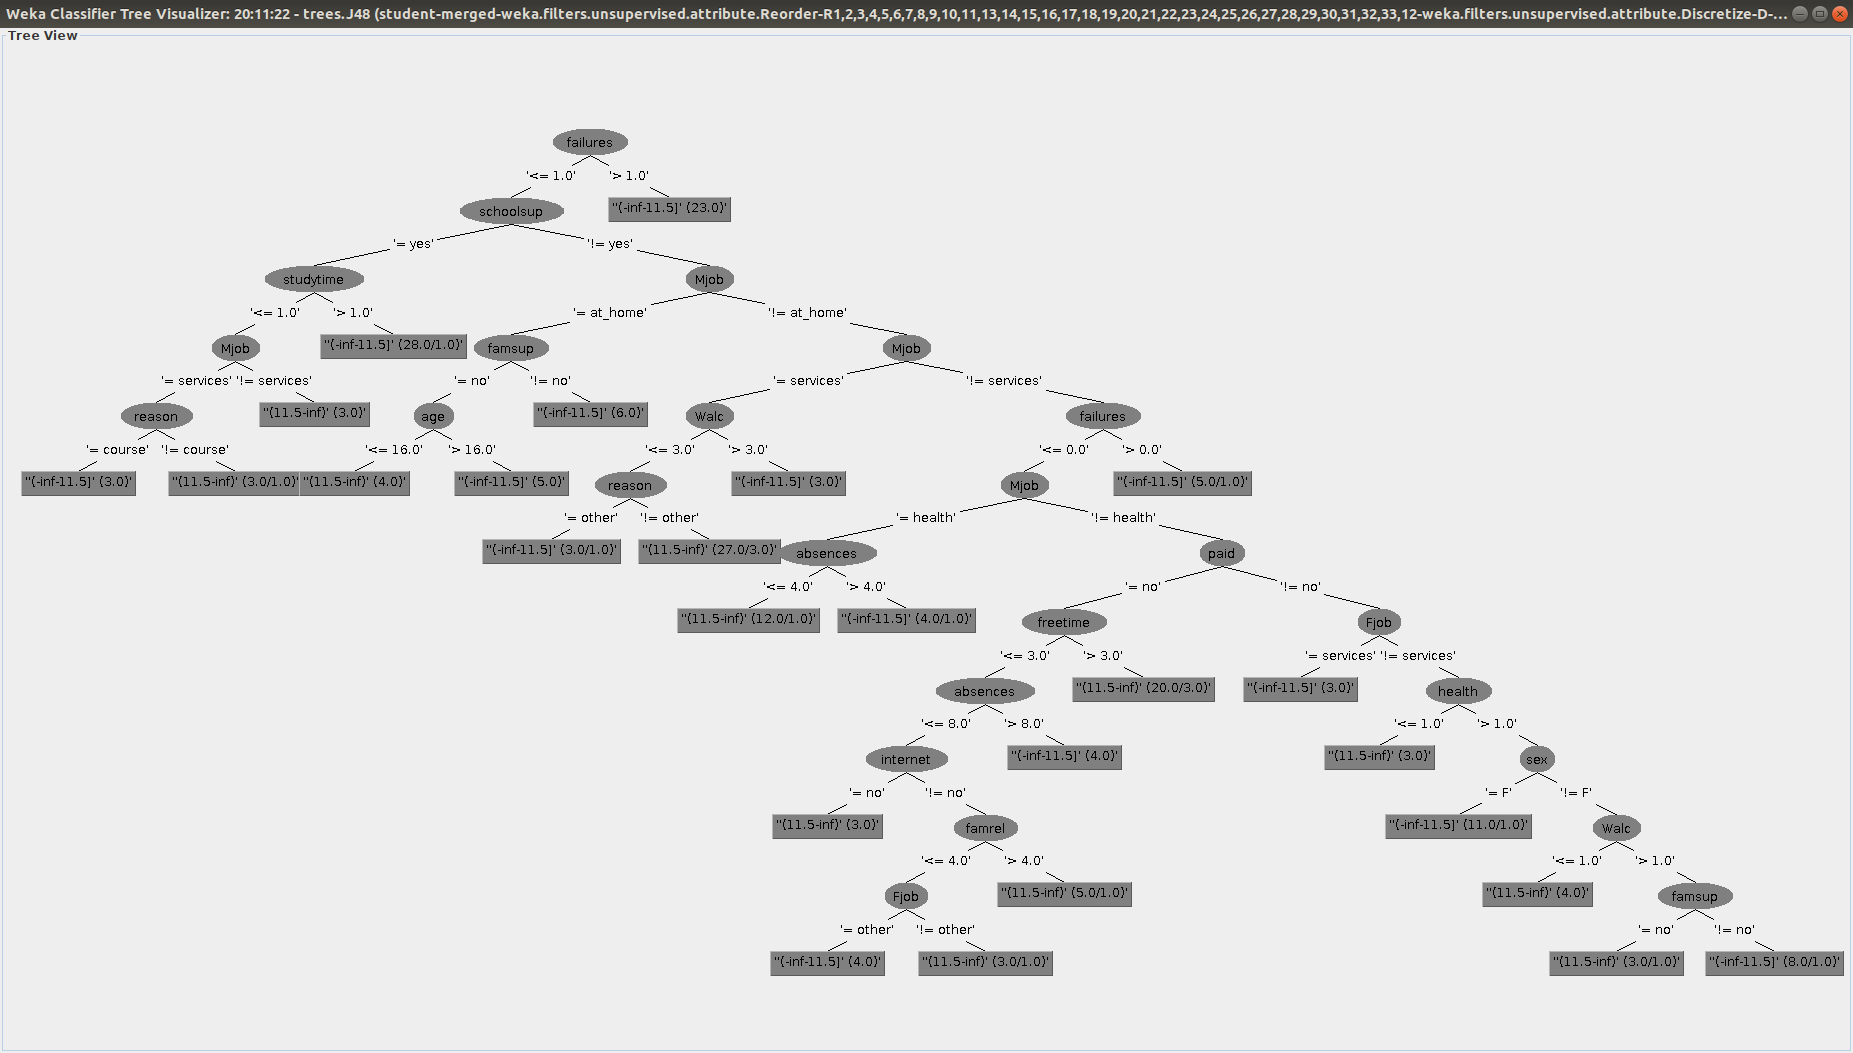
\includegraphics[width=\linewidth]{Drzewo_train_all.png}
	\end{subfigure}
	\label{fig:Chosen}
	\caption{Najlepsze drzewo - ConfidenceFactor=0.5, MinNumbObj=3, BinarySplit=True - zadanie 5.}
\end{figure}

\clearpage
\rowcolors{2}{gray!25}{white}
\begin{table}
	\caption{Porównanie wartości wybranych metryk dla drzew decyzyjnych ewaluowanych z użyciem krzyżowej waldacji - portugal dataset, zadanie 6.}
	\scalebox{0.64}{
		\begin{tabular}{| l | l | l | l | l | l | l | l | l | l |}
			\rowcolor{gray!50}
			\hline
			Binary Split & Confidence factor & Minimum objects & TP & FP & FN & TN & Accuracy & F1 & Balanced Accuracy\\ \hline
			0 & 0.1000 & 2 & 277 & 134 & 71 & 167 & 0.6841 & 0.7299 & 0.6754\\ \hline
			0 & 0.2000 & 2 & 262 & 126 & 86 & 175 & 0.6733 & 0.7120 & 0.6671\\ \hline
			0 & 0.3000 & 2 & 256 & 124 & 92 & 177 & 0.6672 & 0.7033 & 0.6618\\ \hline
			0 & 0.4000 & 2 & 250 & 123 & 98 & 178 & 0.6595 & 0.6935 & 0.6549\\ \hline
			0 & 0.5000 & 2 & 248 & 123 & 100 & 178 & 0.6564 & 0.6898 & 0.6520\\ \hline
			0 & 0.6000 & 2 & 239 & 121 & 109 & 180 & 0.6456 & 0.6751 & 0.6424\\ \hline
			0 & 0.7000 & 2 & 239 & 121 & 109 & 180 & 0.6456 & 0.6751 & 0.6424\\ \hline
			0 & 0.8000 & 2 & 239 & 121 & 109 & 180 & 0.6456 & 0.6751 & 0.6424\\ \hline
			0 & 0.9000 & 2 & 239 & 121 & 109 & 180 & 0.6456 & 0.6751 & 0.6424\\ \hline
			1 & 0.1000 & 2 & 273 & 125 & 75 & 176 & 0.6918 & 0.7319 & 0.6846\\ \hline
			1 & 0.2000 & 2 & 256 & 123 & 92 & 178 & 0.6687 & 0.7043 & 0.6635\\ \hline
			1 & 0.3000 & 2 & 248 & 119 & 100 & 182 & 0.6626 & 0.6937 & 0.6586\\ \hline
			1 & 0.4000 & 2 & 235 & 108 & 113 & 193 & 0.6595 & 0.6802 & 0.6582\\ \hline
			1 & 0.5000 & 2 & 233 & 106 & 115 & 195 & 0.6595 & 0.6783 & 0.6587\\ \hline
			1 & 0.6000 & 2 & 234 & 108 & 114 & 193 & 0.6579 & 0.6783 & 0.6568\\ \hline
			1 & 0.7000 & 2 & 234 & 108 & 114 & 193 & 0.6579 & 0.6783 & 0.6568\\ \hline
			1 & 0.8000 & 2 & 234 & 108 & 114 & 193 & 0.6579 & 0.6783 & 0.6568\\ \hline
			1 & 0.9000 & 2 & 234 & 108 & 114 & 193 & 0.6579 & 0.6783 & 0.6568\\ \hline
			0 & 0.1000 & 3 & 283 & 133 & 65 & 168 & 0.6949 & 0.7408 & 0.6857\\ \hline
			0 & 0.2000 & 3 & 274 & 129 & 74 & 172 & 0.6872 & 0.7297 & 0.6794\\ \hline
			0 & 0.3000 & 3 & 256 & 118 & 92 & 183 & 0.6764 & 0.7091 & 0.6718\\ \hline
			0 & 0.4000 & 3 & 254 & 116 & 94 & 185 & 0.6764 & 0.7075 & 0.6723\\ \hline
			0 & 0.5000 & 3 & 251 & 113 & 97 & 188 & 0.6764 & 0.7051 & 0.6729\\ \hline
			0 & 0.6000 & 3 & 242 & 111 & 106 & 190 & 0.6656 & 0.6904 & 0.6633\\ \hline
			0 & 0.7000 & 3 & 242 & 111 & 106 & 190 & 0.6656 & 0.6904 & 0.6633\\ \hline
			0 & 0.8000 & 3 & 242 & 111 & 106 & 190 & 0.6656 & 0.6904 & 0.6633\\ \hline
			0 & 0.9000 & 3 & 242 & 111 & 106 & 190 & 0.6656 & 0.6904 & 0.6633\\ \hline
			1 & 0.1000 & 3 & 273 & 122 & 75 & 179 & 0.6965 & 0.7349 & 0.6896\\ \hline
			1 & 0.2000 & 3 & 264 & 113 & 84 & 188 & 0.6965 & 0.7283 & 0.6916\\ \hline
			1 & 0.3000 & 3 & 257 & 110 & 91 & 191 & 0.6903 & 0.7189 & 0.6865\\ \hline
			1 & 0.4000 & 3 & 248 & 105 & 100 & 196 & 0.6841 & 0.7076 & 0.6819\\ \hline
			1 & 0.5000 & 3 & 248 & 103 & 100 & 198 & 0.6872 & 0.7096 & 0.6852\\ \hline
			1 & 0.6000 & 3 & 245 & 105 & 103 & 196 & 0.6795 & 0.7020 & 0.6776\\ \hline
			1 & 0.7000 & 3 & 245 & 105 & 103 & 196 & 0.6795 & 0.7020 & 0.6776\\ \hline
			1 & 0.8000 & 3 & 245 & 105 & 103 & 196 & 0.6795 & 0.7020 & 0.6776\\ \hline
			1 & 0.9000 & 3 & 245 & 105 & 103 & 196 & 0.6795 & 0.7020 & 0.6776\\ \hline
			0 & 0.1000 & 4 & 286 & 136 & 62 & 165 & 0.6949 & 0.7429 & 0.6850\\ \hline
			0 & 0.2000 & 4 & 275 & 133 & 73 & 168 & 0.6826 & 0.7275 & 0.6742\\ \hline
			0 & 0.3000 & 4 & 266 & 121 & 82 & 180 & 0.6872 & 0.7238 & 0.6812\\ \hline
			0 & 0.4000 & 4 & 263 & 117 & 85 & 184 & 0.6888 & 0.7225 & 0.6835\\ \hline
			0 & 0.5000 & 4 & 261 & 117 & 87 & 184 & 0.6857 & 0.7190 & 0.6806\\ \hline
			0 & 0.6000 & 4 & 245 & 113 & 103 & 188 & 0.6672 & 0.6941 & 0.6643\\ \hline
			0 & 0.7000 & 4 & 245 & 113 & 103 & 188 & 0.6672 & 0.6941 & 0.6643\\ \hline
			0 & 0.8000 & 4 & 245 & 113 & 103 & 188 & 0.6672 & 0.6941 & 0.6643\\ \hline
			0 & 0.9000 & 4 & 245 & 113 & 103 & 188 & 0.6672 & 0.6941 & 0.6643\\ \hline
			1 & 0.1000 & 4 & 271 & 127 & 77 & 174 & 0.6857 & 0.7265 & 0.6784\\ \hline
			1 & 0.2000 & 4 & 269 & 125 & 79 & 176 & 0.6857 & 0.7251 & 0.6789\\ \hline
			1 & 0.3000 & 4 & 252 & 120 & 96 & 181 & 0.6672 & 0.7000 & 0.6627\\ \hline
			1 & 0.4000 & 4 & 247 & 110 & 101 & 191 & 0.6749 & 0.7007 & 0.6722\\ \hline
			1 & 0.5000 & 4 & 245 & 108 & 103 & 193 & 0.6749 & 0.6990 & 0.6726\\ \hline
			1 & 0.6000 & 4 & 237 & 109 & 111 & 192 & 0.6610 & 0.6830 & 0.6595\\ \hline
			1 & 0.7000 & 4 & 237 & 109 & 111 & 192 & 0.6610 & 0.6830 & 0.6595\\ \hline
			1 & 0.8000 & 4 & 237 & 109 & 111 & 192 & 0.6610 & 0.6830 & 0.6595\\ \hline
			1 & 0.9000 & 4 & 237 & 109 & 111 & 192 & 0.6610 & 0.6830 & 0.6595\\ \hline
			0 & 0.1000 & 5 & 288 & 137 & 60 & 164 & 0.6965 & 0.7451 & 0.6862\\ \hline
			0 & 0.2000 & 5 & 274 & 128 & 74 & 173 & 0.6888 & 0.7307 & 0.6811\\ \hline
			0 & 0.3000 & 5 & 257 & 119 & 91 & 182 & 0.6764 & 0.7099 & 0.6716\\ \hline
			0 & 0.4000 & 5 & 252 & 115 & 96 & 186 & 0.6749 & 0.7049 & 0.6710\\ \hline
			0 & 0.5000 & 5 & 252 & 112 & 96 & 189 & 0.6795 & 0.7079 & 0.6760\\ \hline
			0 & 0.6000 & 5 & 234 & 109 & 114 & 192 & 0.6564 & 0.6773 & 0.6551\\ \hline
			0 & 0.7000 & 5 & 234 & 109 & 114 & 192 & 0.6564 & 0.6773 & 0.6551\\ \hline
			0 & 0.8000 & 5 & 234 & 109 & 114 & 192 & 0.6564 & 0.6773 & 0.6551\\ \hline
			0 & 0.9000 & 5 & 234 & 109 & 114 & 192 & 0.6564 & 0.6773 & 0.6551\\ \hline
			1 & 0.1000 & 5 & 282 & 129 & 66 & 172 & 0.6995 & 0.7431 & 0.6909\\ \hline
			1 & 0.2000 & 5 & 268 & 124 & 80 & 177 & 0.6857 & 0.7243 & 0.6791\\ \hline
			1 & 0.3000 & 5 & 263 & 124 & 85 & 177 & 0.6780 & 0.7156 & 0.6719\\ \hline
			1 & 0.4000 & 5 & 258 & 120 & 90 & 181 & 0.6764 & 0.7107 & 0.6714\\ \hline
			1 & 0.5000 & 5 & 255 & 119 & 93 & 182 & 0.6733 & 0.7064 & 0.6687\\ \hline
			1 & 0.6000 & 5 & 240 & 116 & 108 & 185 & 0.6549 & 0.6818 & 0.6521\\ \hline
			1 & 0.7000 & 5 & 240 & 116 & 108 & 185 & 0.6549 & 0.6818 & 0.6521\\ \hline
			1 & 0.8000 & 5 & 240 & 116 & 108 & 185 & 0.6549 & 0.6818 & 0.6521\\ \hline
			1 & 0.9000 & 5 & 240 & 116 & 108 & 185 & 0.6549 & 0.6818 & 0.6521\\ \hline
			
		\end{tabular}
	}
\end{table}
\clearpage
\begin{figure}[h!]
	\centering
	\begin{subfigure}[b]{1\linewidth}
		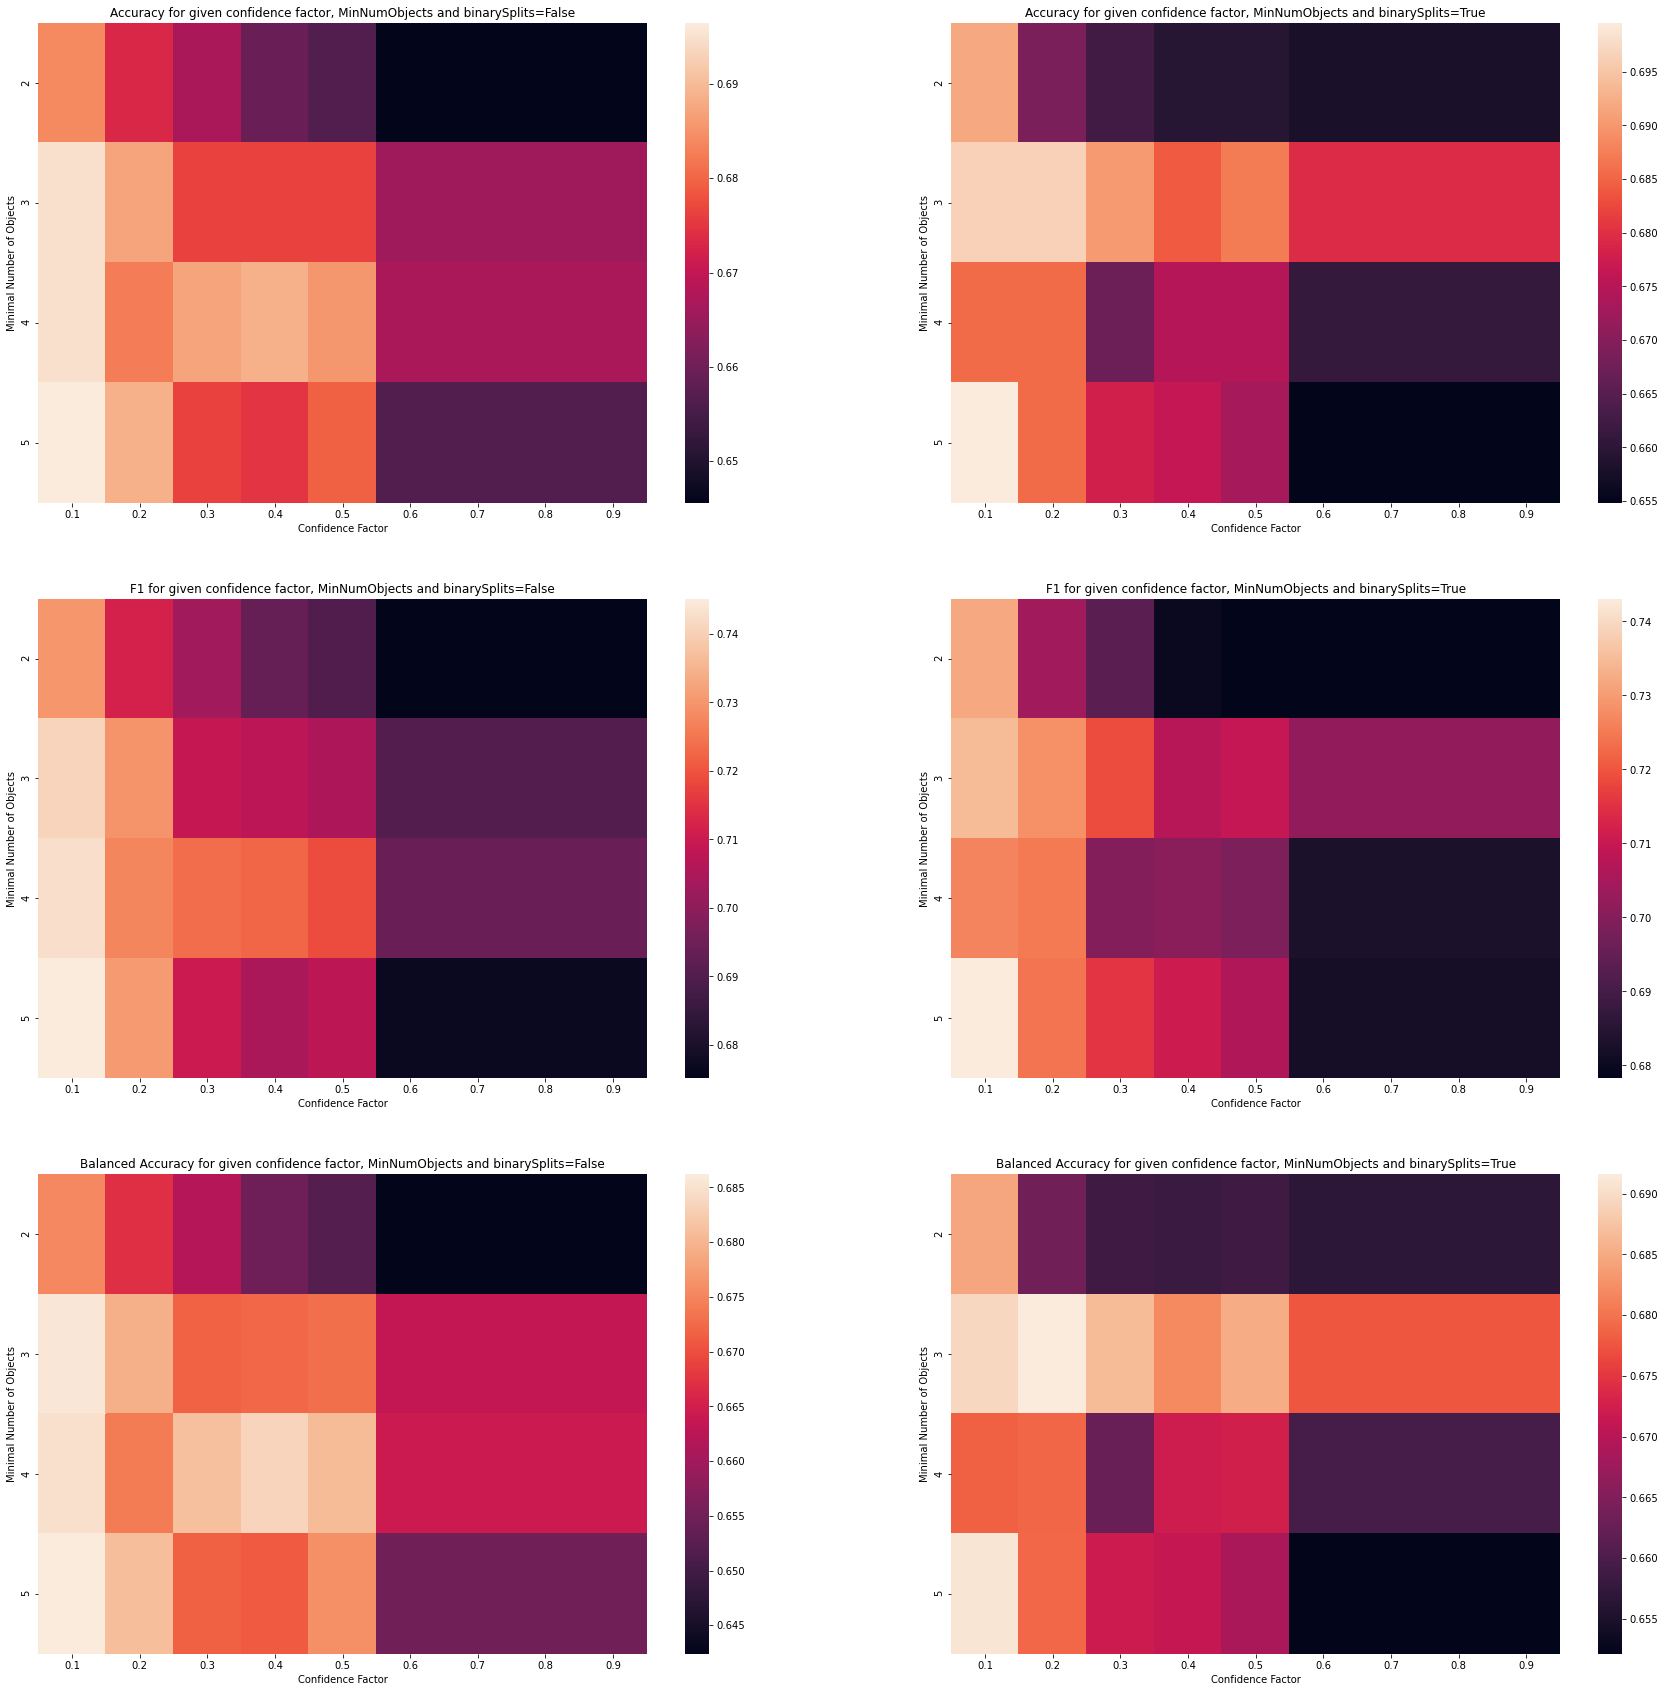
\includegraphics[width=\linewidth]{Port_all.png}
	\end{subfigure}
	\label{fig:dyskretne}
	\caption{Wartość kolejnych metryk w zależności od hiperparametrów: Confidence factor i Minimum number of objects (in a leaf) - zadanie 6.}
\end{figure}

\clearpage
\begin{figure}[h!]
	\centering
	\begin{subfigure}[b]{1\linewidth}
		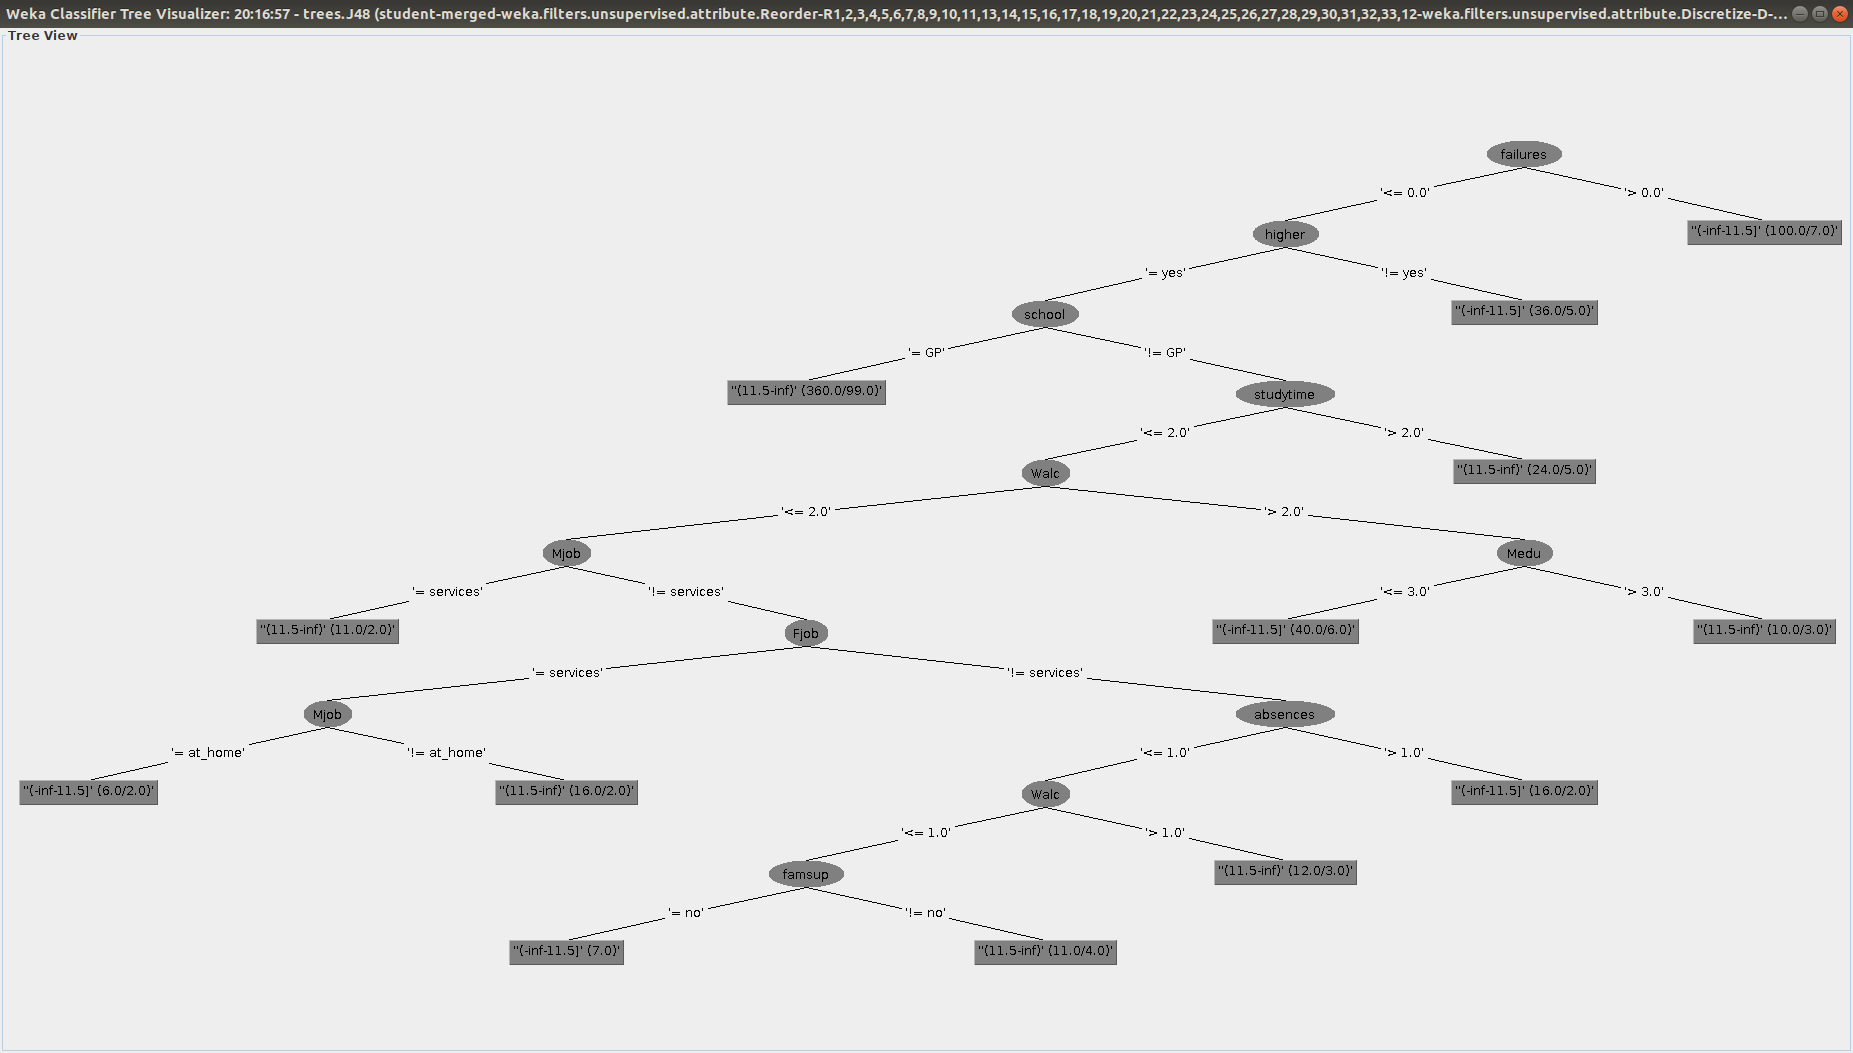
\includegraphics[width=\linewidth]{Drzewo_port.png}
	\end{subfigure}
	\label{fig:Chosen}
	\caption{Najlepsze drzewo - ConfidenceFactor=0.1, MinNumbObj=5, BinarySplit=True - zadanie 6.}
\end{figure}
\clearpage

\section{Powiązania między drzewami, podobieństwa, zasadność pierwotnie wybranych atrybutów}
\begin{enumerate}
	\item W każdym drzewie liczba poprzednich porażek w przejściu do następnej klasy była pierwszym predyktorem tego, czy ktoś zdał przedmiot - był to argument wybrany na początku, jeden z siedmiu.
	\item Najlepsze drzewa używające wszystkich atrybutów poza pierwszym używały jako predyktora Weekend Alcohol Consumption raczej niż Workday alcohol consumption, czyli drugiego z wykorzystanych w pierwszym modelu atrybutów.
	\item Co ciekawe chęć podjęcia edukacji wyższej miała duży wpływ na drzewo decyzyjne dla ocen z języka portugalskiego, ale zerowy dla matematyki (dla wszystkich atrybutów)
	\item Pozostałe atrybuty wybrane pierwotnie (płeć, zdrowie, przyczyny, absencje) były wykorzystywane na niższych poziomach pozostałych drzewa decyzyjnego dotyczącego matematyki (dla portugalskiego tylko absences, i to na niskim poziomie drzewa)
	\item Oba drzewa korzystające ze wszystkich atrybutów używały jako kluczowych atrybutów (na najwyższych poziomach drzewa) czasu nauki w tygodniu, a także branż w jakich pracują ojciec/matka
	\item Dodatkowo drzewo predykcji ocen z matematyki używało wsparcia (czyli zapewne korepetycji etc.) jako jednego z głównych predyktorów
	\item Bazując na tych rezultatach nie można powiedzieć absolutnie nic o tym, czy uczeń jest uważny w szkole - te dane nie dają podstaw, by wierzyć, że istnieje korelacja między uważnością, a oceną z matematyki/portugalskiego, a jeśli istnieje, to w którą stronę - na gruncie czysto racjonalnym można argumentować, że uczeń uważny będzie słuchał na zajęciach i otrzyma wyższą ocenę, można też argumentować, że potężny matematyk/poeta nie będzie się zajmował na zajęciach z tych przedmiotów jakimiś śmiesznymi, plebejskimi, niezniuansowanymi, ludzkimi, arcyludzkimi problemami/poematami, zamiast tego zajmując się swoimi, po wielokroć ciekawszymi sprawami - a i tak dostanie najwyższą możliwą ocenę.
	\item Jeśli natomiast pytanie "Basing on these results, can we say
	which attributes can say if the student is attentive?" było o ocenę ucznia w zależności od tych atrybutów, to najlepszymi predyktorami oceny wydają się:
	\begin{enumerate}
		\item Liczba poprzednich niezdanych lat/przedmiotów
		\item Praca matki
		\item Praca ojca
		\item Czas nauki
		\item Spożycie alkoholu w weekend
		\item Dla matematyki - Wsparcie szkolne (korepetycje), dla portugalskiego - wybrana szkoła
	\end{enumerate}
\end{enumerate}

\section{Zasadność pierwotnie wybranych atrybutów w kontekście Naive Bayesa}
Patrząc na Przynależność do klas w zależności od atrybutów w algorytmie Bayesa, zasadnymi predyktorami (wybrane 7) są atrybuty:
\begin{enumerate}
	\item Weekend Alcohol consumption in workdays - nieuwzględniony na początku
	\item Higher - uwzględniony na początku
	\item Failures - uwzględniony na początku
	\item Sex - uwzględniony na początku
	\item Mjob - nieuwzględniony na początku
	\item Reason - uwzględniony na początku
	\item School Support - nieuwzględniony na początku
\end{enumerate}


\end{document}
